\textbf{Creación de Máquina Virtual}
\begin{enumerate}
\item Test.
\begin{figure}[H] %[H] para here [b] para bottom [t] para top
\begin{center}
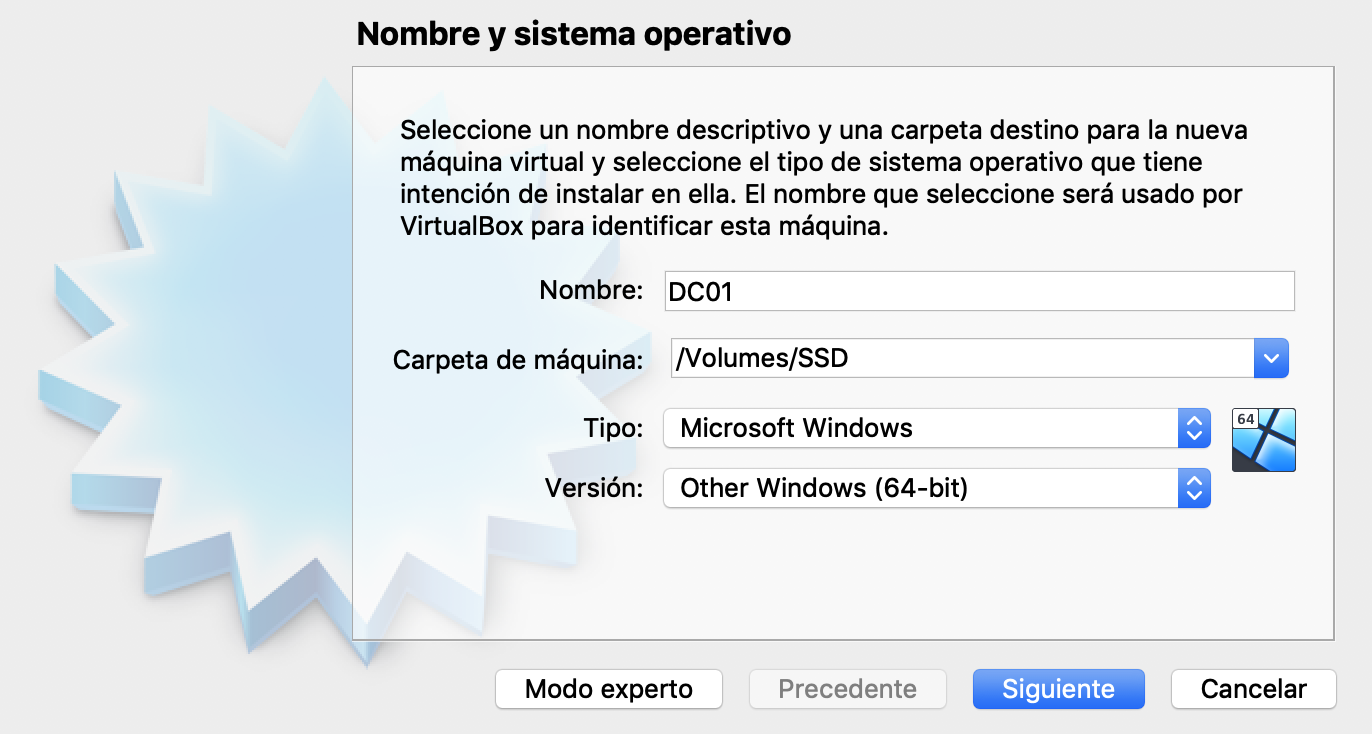
\includegraphics[width=10cm]{DC01/MV1.png}
\end{center}
\end{figure}

\item Test
\begin{figure}[H] %[H] para here [b] para bottom [t] para top
\begin{center}
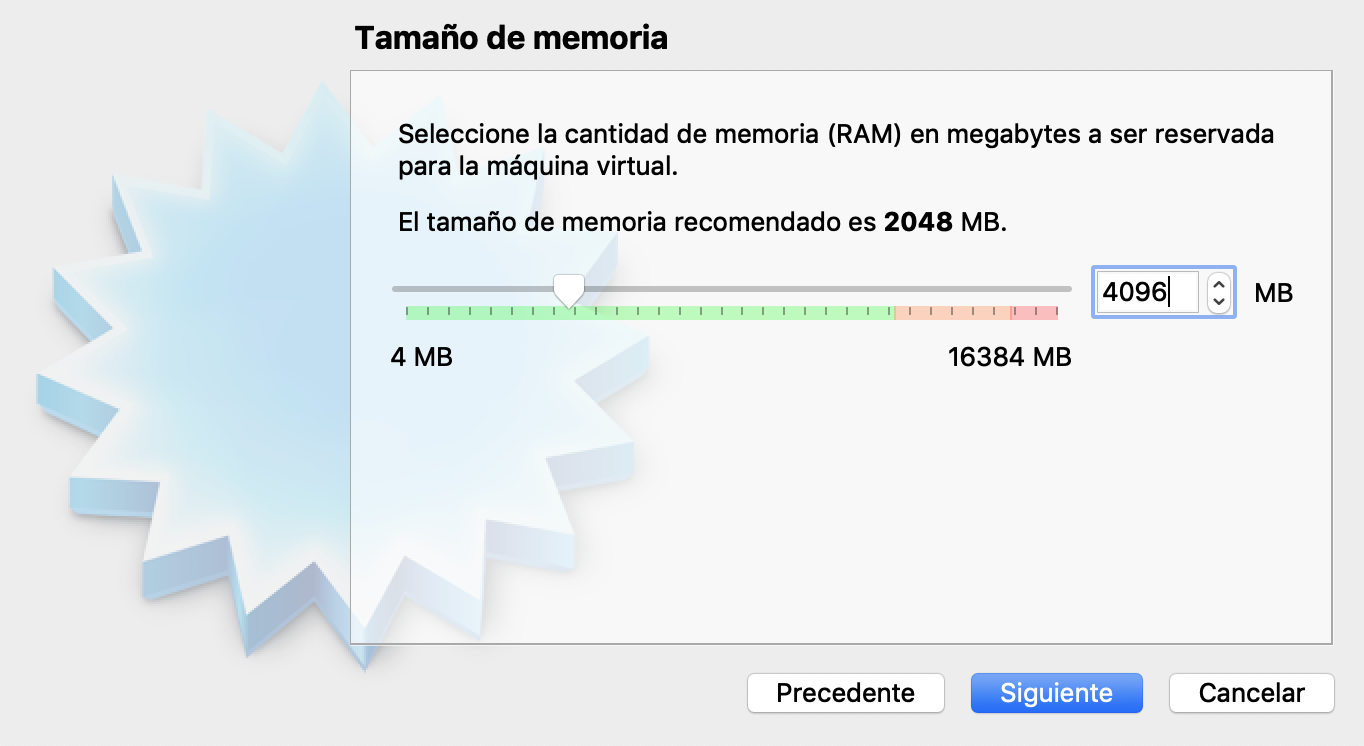
\includegraphics[width=10cm]{DC01/MV2.png}
\end{center}
\end{figure}

\item Test
\begin{figure}[H] %[H] para here [b] para bottom [t] para top
\begin{center}
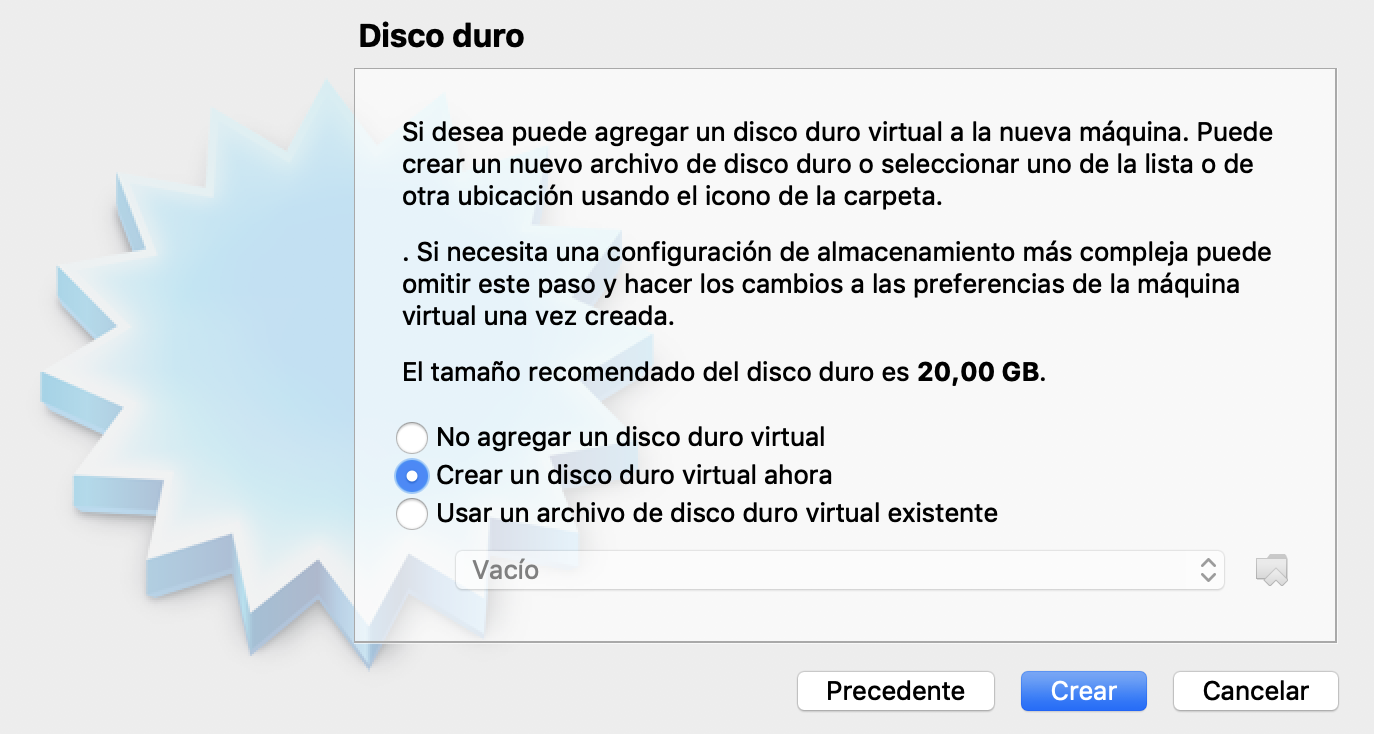
\includegraphics[width=10cm]{DC01/MV3.png}
\end{center}
\end{figure}

\item Test
\begin{figure}[H] %[H] para here [b] para bottom [t] para top
\begin{center}
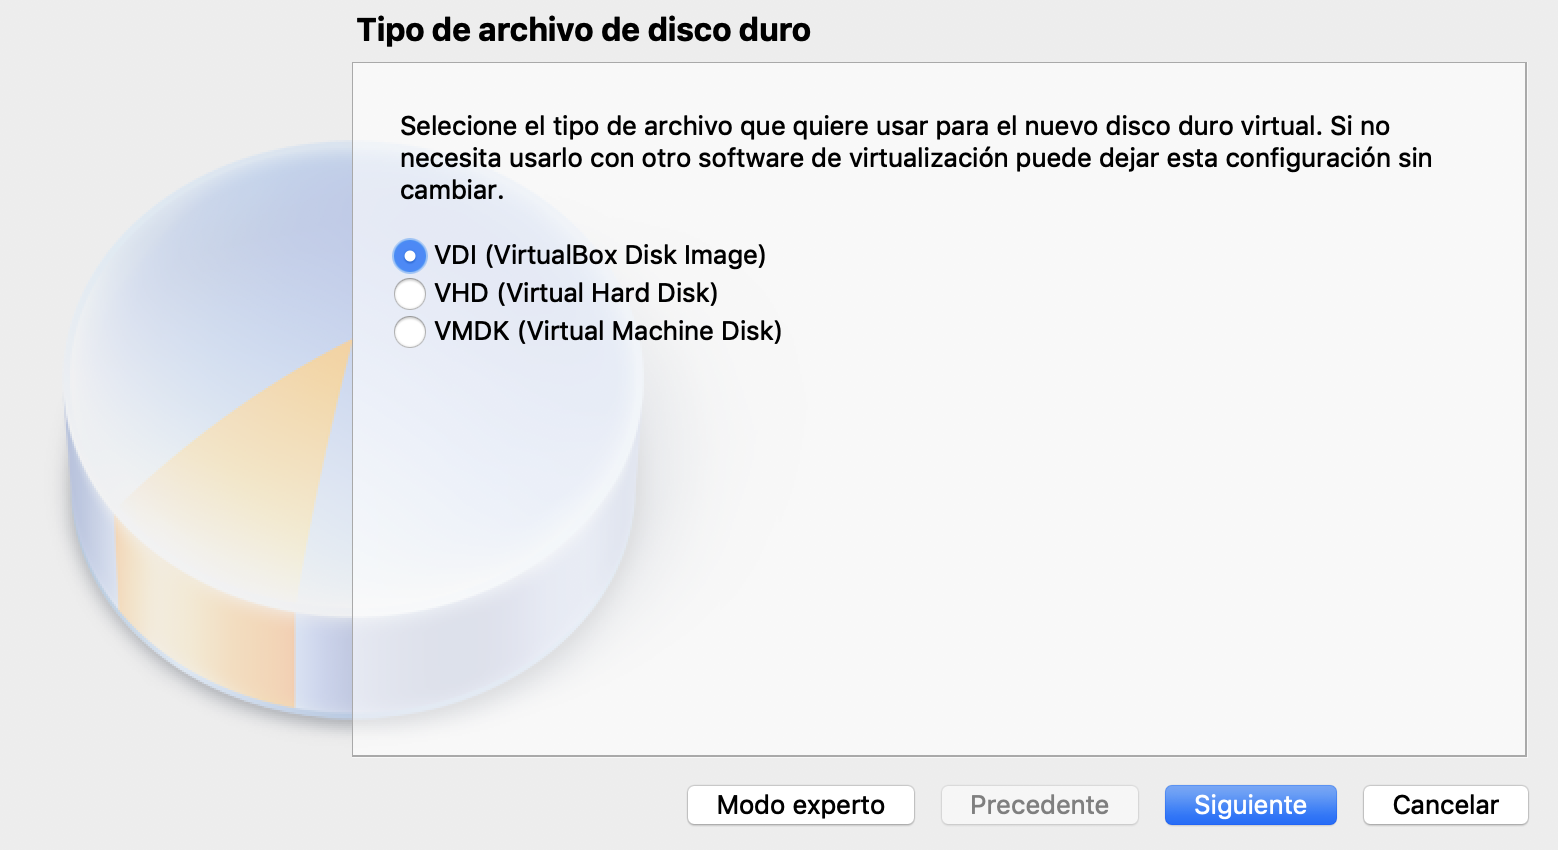
\includegraphics[width=10cm]{DC01/MV4.png}
\end{center}
\end{figure}

\item Test
\begin{figure}[H] %[H] para here [b] para bottom [t] para top
\begin{center}
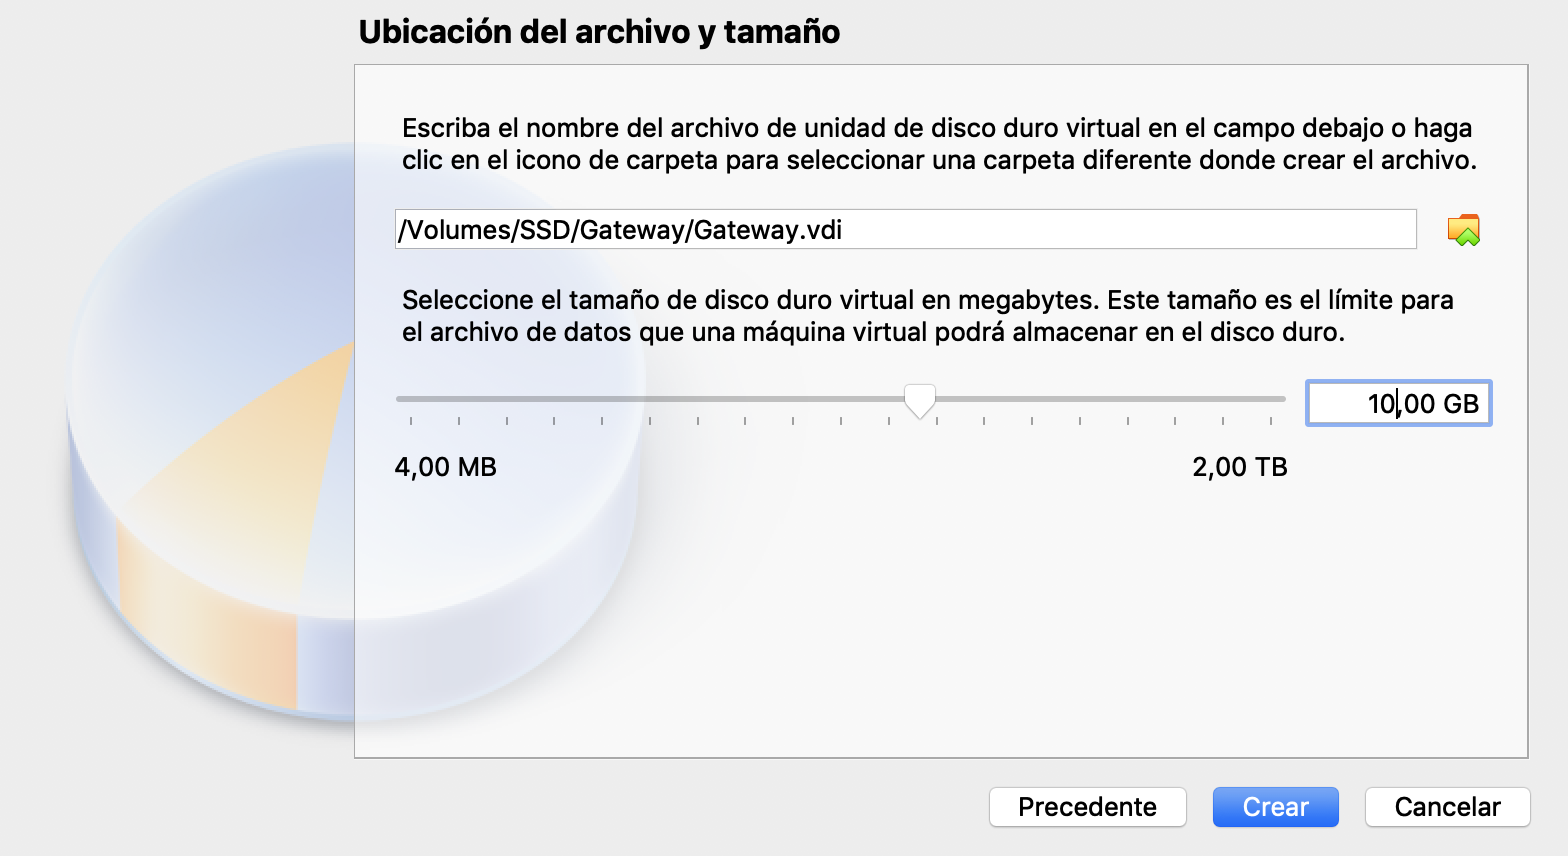
\includegraphics[width=10cm]{DC01/MV5.png}
\end{center}
\end{figure}

\item Test
\begin{figure}[H] %[H] para here [b] para bottom [t] para top
\begin{center}
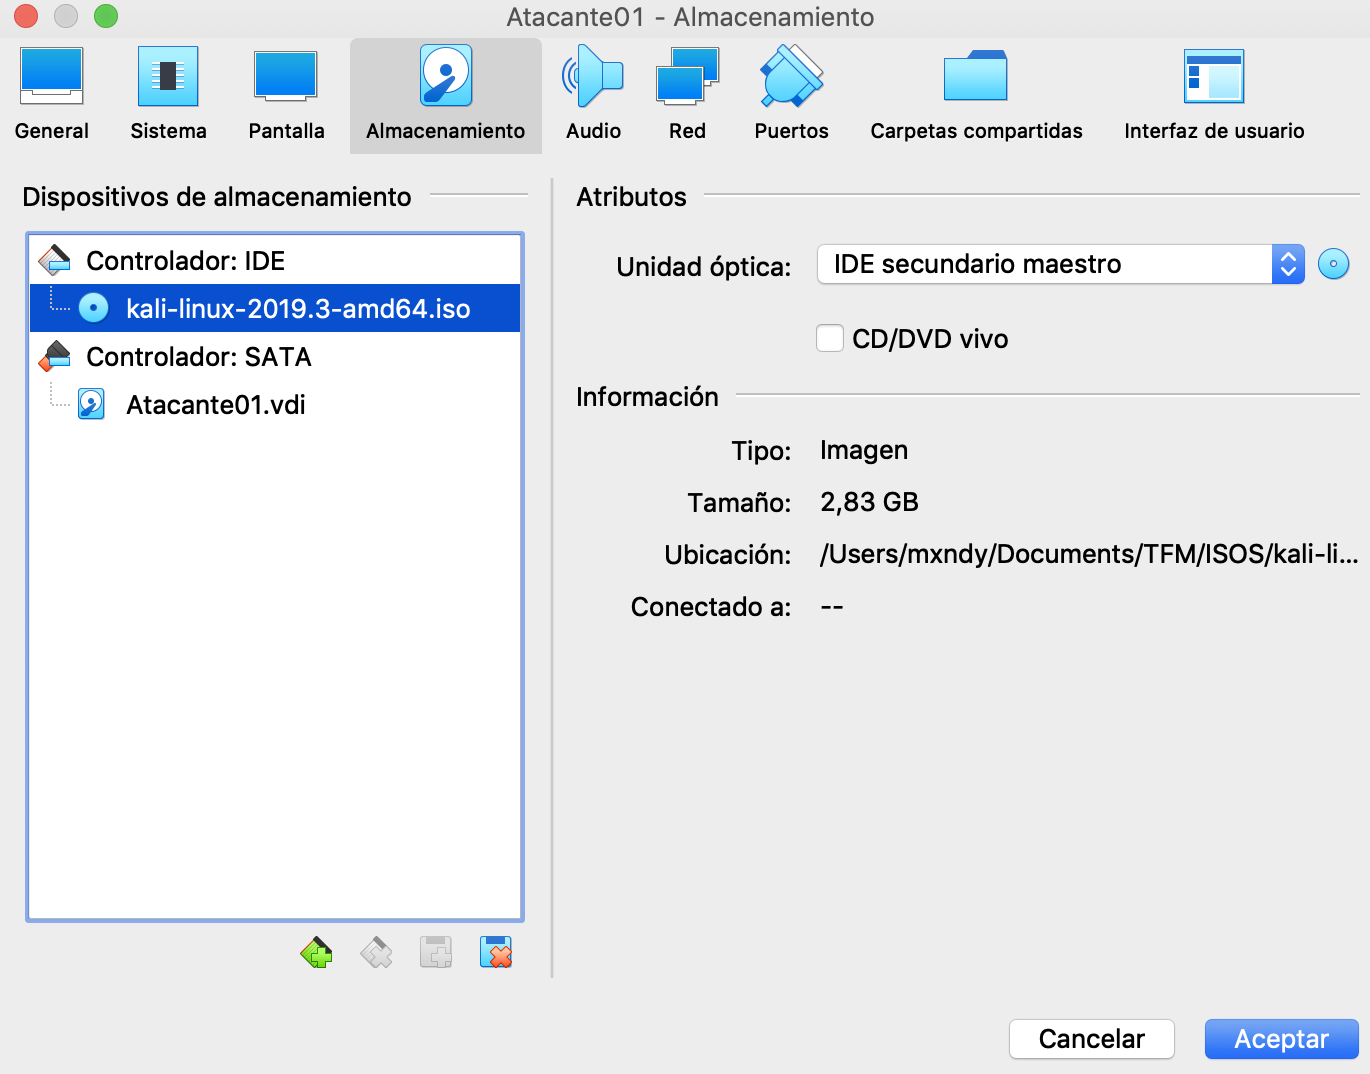
\includegraphics[width=10cm]{DC01/MV6.png}
\end{center}
\end{figure}

\item Test
\begin{figure}[H] %[H] para here [b] para bottom [t] para top
\begin{center}
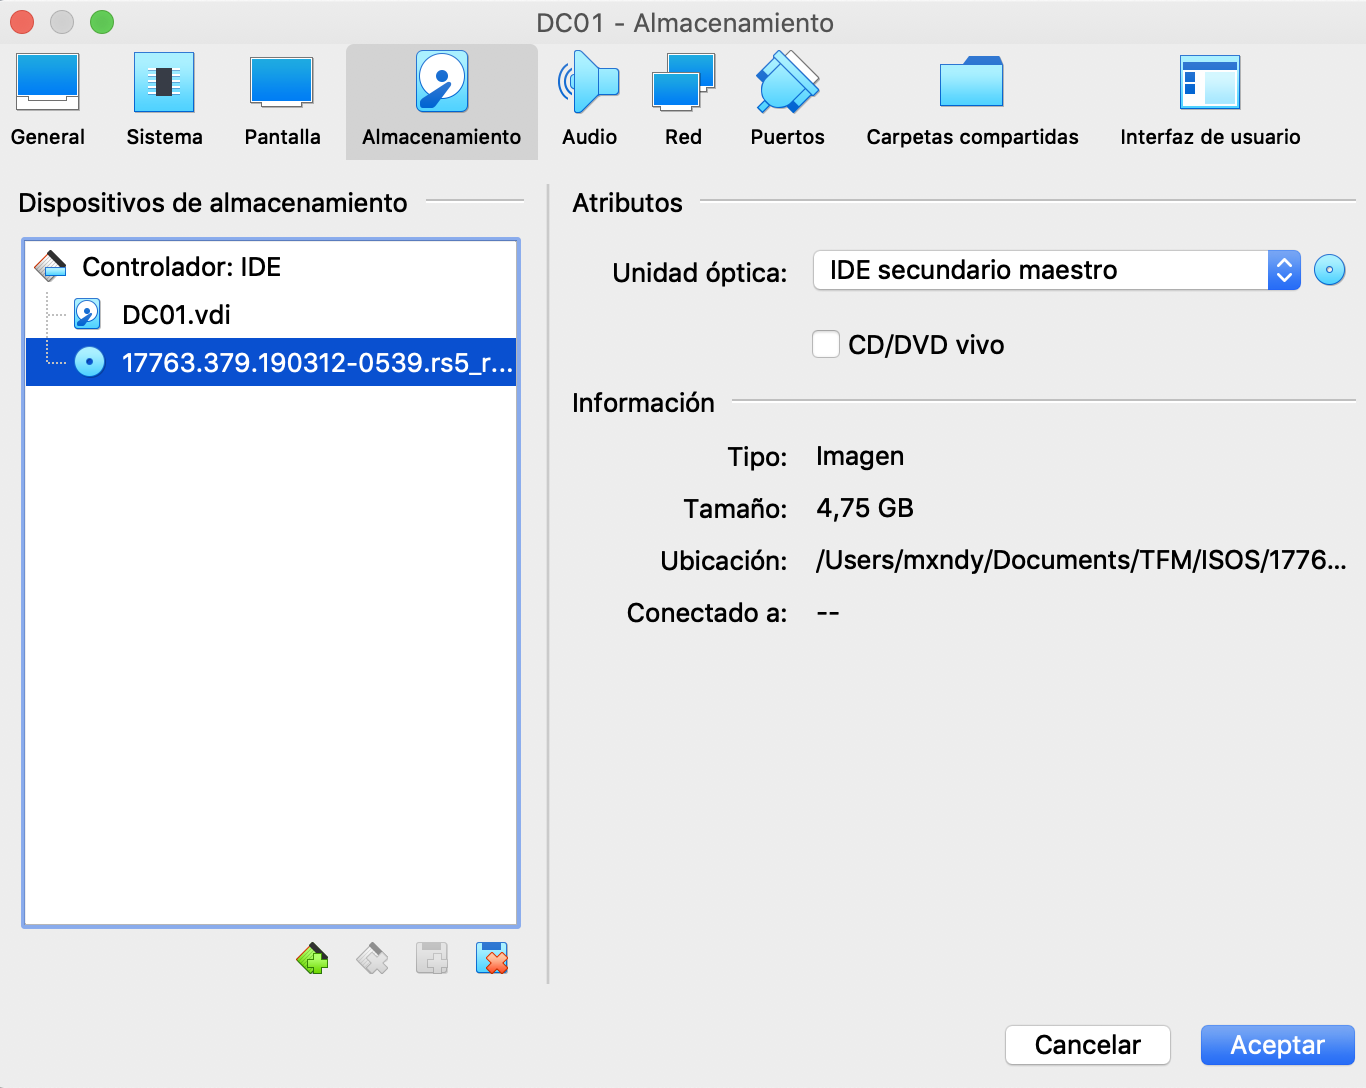
\includegraphics[width=10cm]{DC01/MV7.png}
\end{center}
\end{figure}

\end{enumerate}



\textbf{Instalación}

\begin{enumerate}
\item Una vez creada la máquina virtual se ejecuta la instacia y se procede a la instalación.
\item En primer lugar, se elige el idioma y el teclado a utilizar. En este caso se ha utilizado la imagen (iso) de Windows Server 2019 en inglés: English (United States) y el teclado en español: Spanish (Spain, International Sort) y spanish como método de entrada.

\begin{figure}[H] %[H] para here [b] para bottom [t] para top
\begin{center}
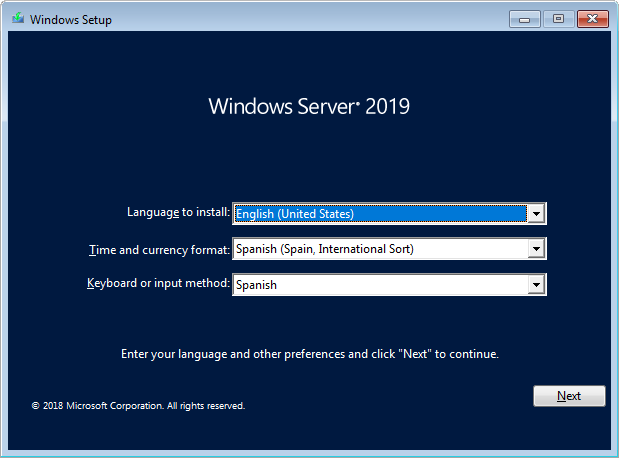
\includegraphics[width=10cm]{DC01/Instalacion1.png}
\end{center}
\end{figure}

\item Se empieza con la instalación pulsando en ``Install Now''.

\begin{figure}[H] %[H] para here [b] para bottom [t] para top
\begin{center}
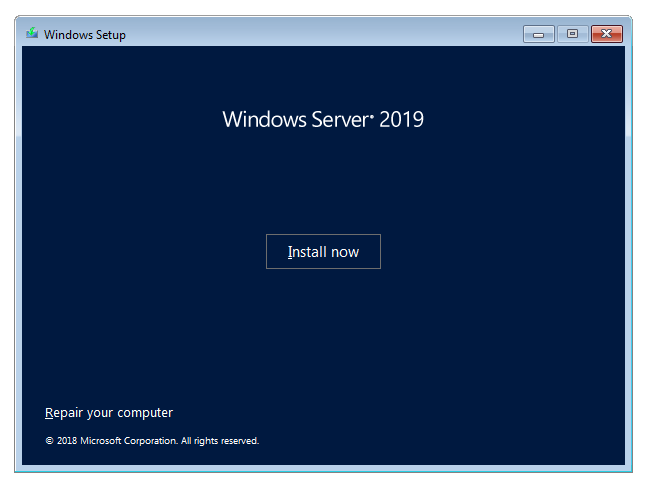
\includegraphics[width=10cm]{DC01/Instalacion2.png}
\end{center}
\end{figure}


\item Test

\begin{figure}[H] %[H] para here [b] para bottom [t] para top
\begin{center}
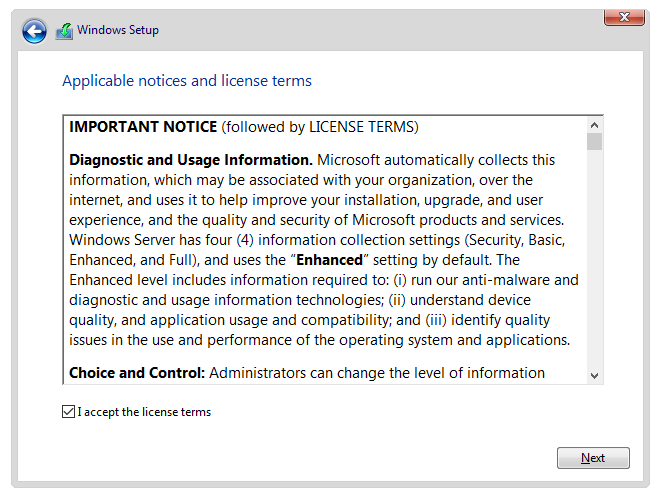
\includegraphics[width=10cm]{DC01/Instalacion3.png}
\end{center}
\end{figure}

\item Test

\begin{figure}[H] %[H] para here [b] para bottom [t] para top
\begin{center}
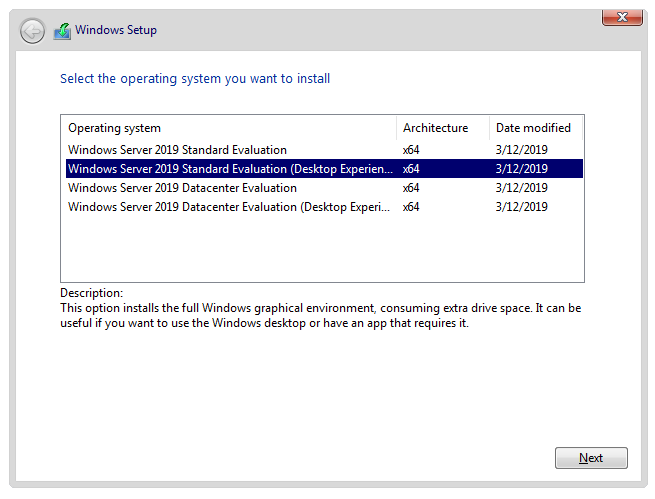
\includegraphics[width=10cm]{DC01/Instalacion4.png}
\end{center}
\end{figure}

\item Test

\begin{figure}[H] %[H] para here [b] para bottom [t] para top
\begin{center}
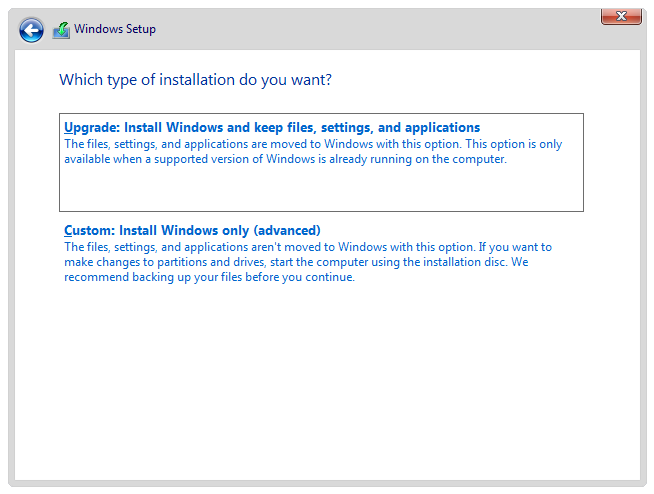
\includegraphics[width=10cm]{DC01/Instalacion5.png}
\end{center}
\end{figure}

\item Test

\begin{figure}[H] %[H] para here [b] para bottom [t] para top
\begin{center}
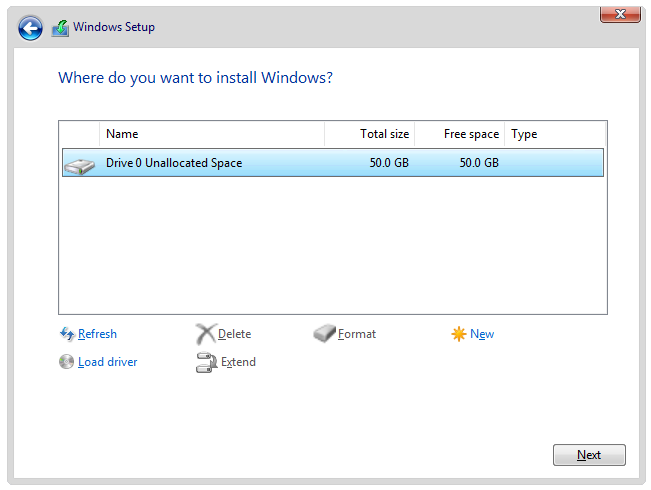
\includegraphics[width=10cm]{DC01/Instalacion6.png}
\end{center}
\end{figure}

\item Test

\begin{figure}[H] %[H] para here [b] para bottom [t] para top
\begin{center}
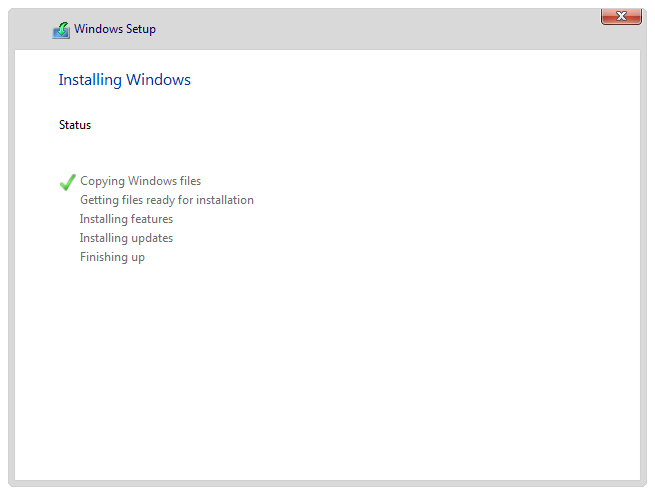
\includegraphics[width=10cm]{DC01/Instalacion7.png}
\end{center}
\end{figure}

\item Test

\begin{figure}[H] %[H] para here [b] para bottom [t] para top
\begin{center}
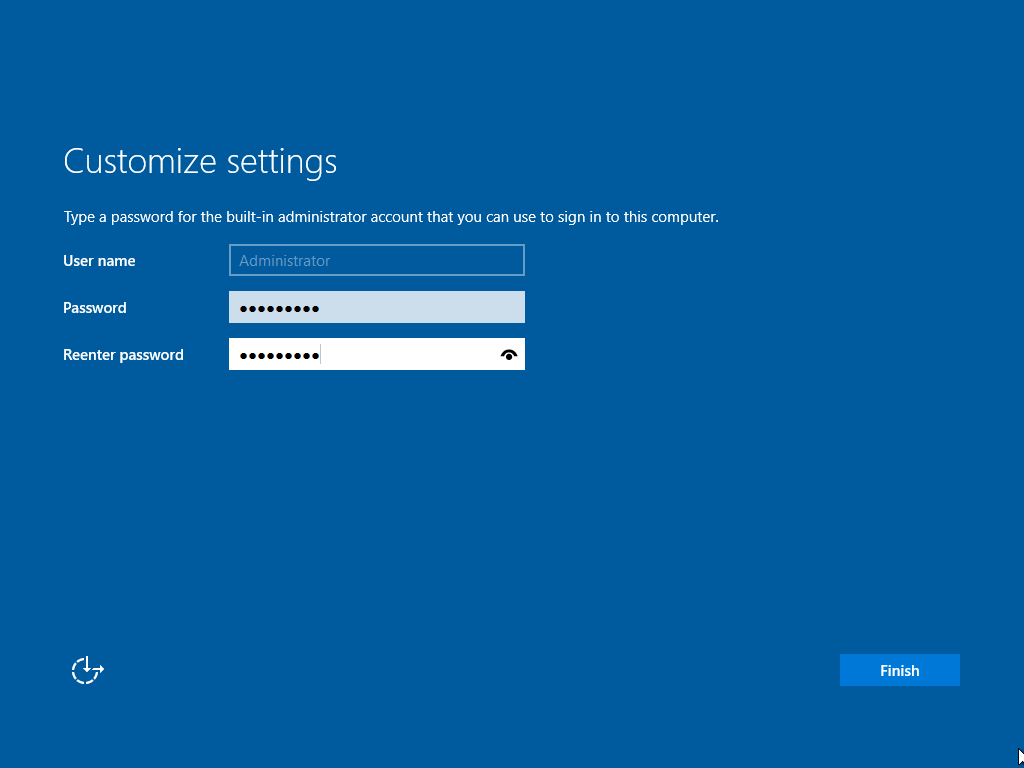
\includegraphics[width=10cm]{DC01/Instalacion8.png}
\end{center}
\end{figure}

\end{enumerate}


\textbf{Actualización}

\begin{enumerate}
\item Test

\begin{figure}[H] %[H] para here [b] para bottom [t] para top
\begin{center}
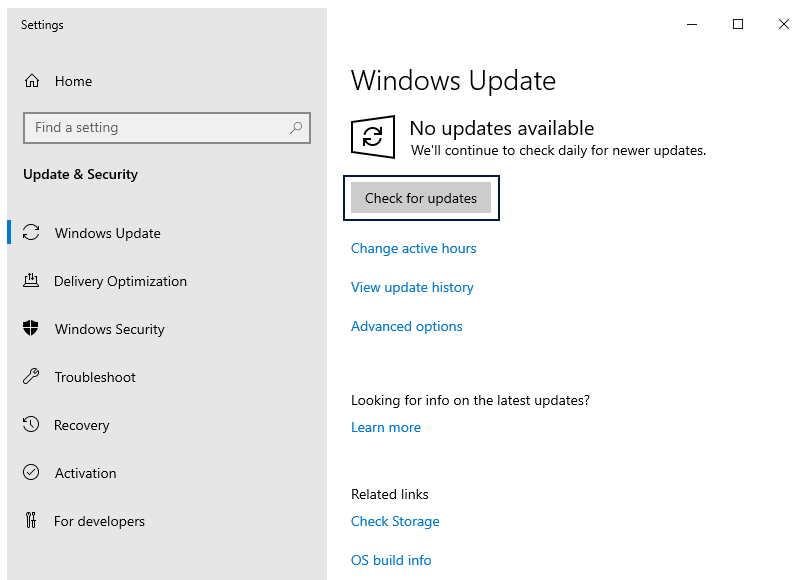
\includegraphics[width=10cm]{DC01/Update1.png}
\end{center}
\end{figure}

\item Test

\begin{figure}[H] %[H] para here [b] para bottom [t] para top
\begin{center}
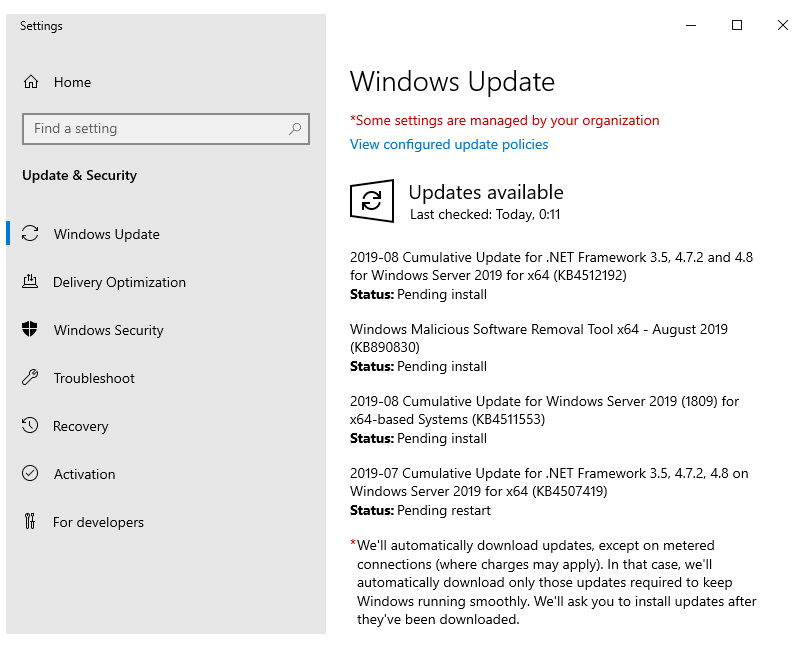
\includegraphics[width=10cm]{DC01/Update2.png}
\end{center}
\end{figure}

\end{enumerate}

\textbf{Configuración}


